\genHeader

{\scriptsize \texttt{Approximate time to complete: ?? minutes} }

% Rewrite and expand!
In this part, we introduce unidirectional model transformations via programmed graph transformations using Story Driven Modeling (SDM). We will be implementing
the methods signatures declared as part of the system's static semantics. It other words, we'll be building dynamic semantics! Don't let the sheer
size of this part frighten you off - We've included deep, thorough explanations and an ample number of messages to ensure clarity. It's really not so bad.

If you're just joining us, read the remainder of this section for a brief overview of the example so far and how to download the files that will let you start right away. 
If you're continuing from Part II, click the link below to continue with your fully-constructed learning box model.

\begin{center}\texttt{$\triangleright$ \hyperlink{explanation}{Continue from Part II\ldots}}\end{center}

\section{Leitner's learning box reviewed}

\emph{Leitner's learning box}\footnote{\href{http://en.wikipedia.org/wiki/Leitner\_system}{http://en.wikipedia.org/wiki/Leitner\_system}} is a simple, but
ingenious little contraption to support the tedious process of memorization, especially prominent when trying to learn, for example, a new language. As depicted in
Fig.~\ref{fig:membox_depiction}, this box consists of a series of partitions with a strict set of rules. The contents to be memorized are written on little cards and placed in the first container. Every
time the user correctly answers a card, that card is promoted to the next partition. Once it reaches the final partition, it can be considered memorized, and
no longer needs to be practiced. Every time the user incorrectly answers a card however, it is returned to the original starting partition, and the
learning process is restarted.

\begin{figure}[htbp]
	\centering
  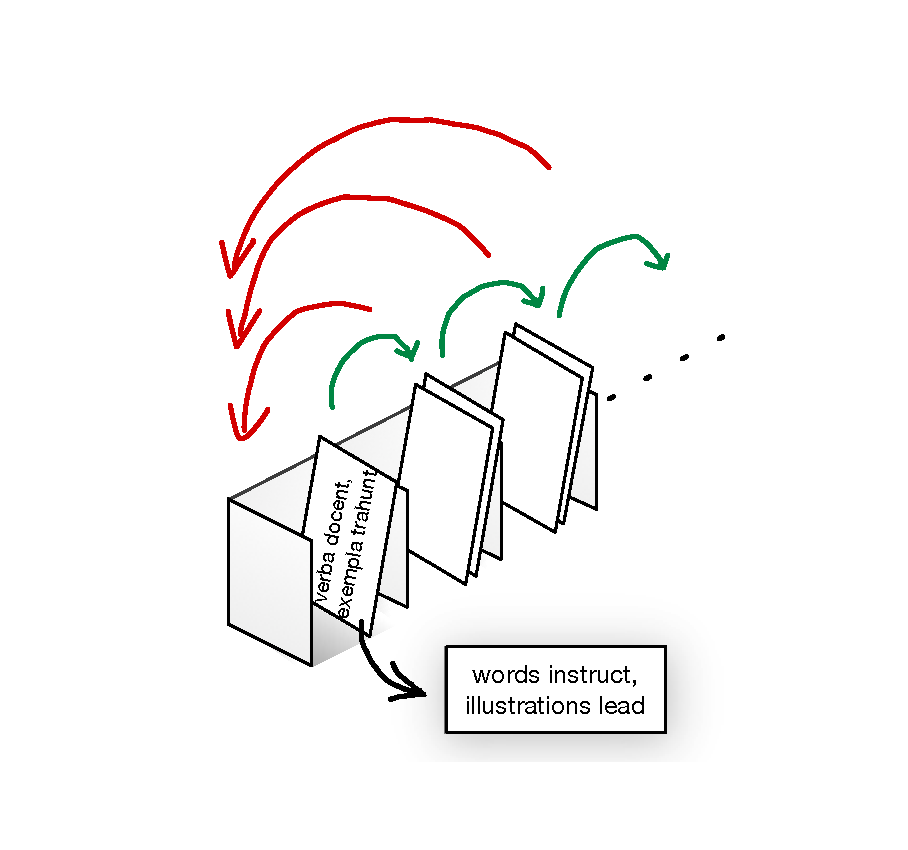
\includegraphics[width=0.4\textwidth]{membox_illustration.pdf}
	\caption{Static Structure of a Leitner's Learning Box}
	\label{fig:membox_depiction}
\end{figure}

For a more detailed overview of the box and our goals, we recommend you read the introduction to Part II. But for now, enough discussion!

\begin{itemize}

\item[$\blacktriangleright$] To get started, press the \texttt{new} button and navigate to ``Examples/eMoflon Handbook Examples/''
(Fig.~\ref{fig:downloadWizard}).

\begin{figure}[htbp]
	\centering
  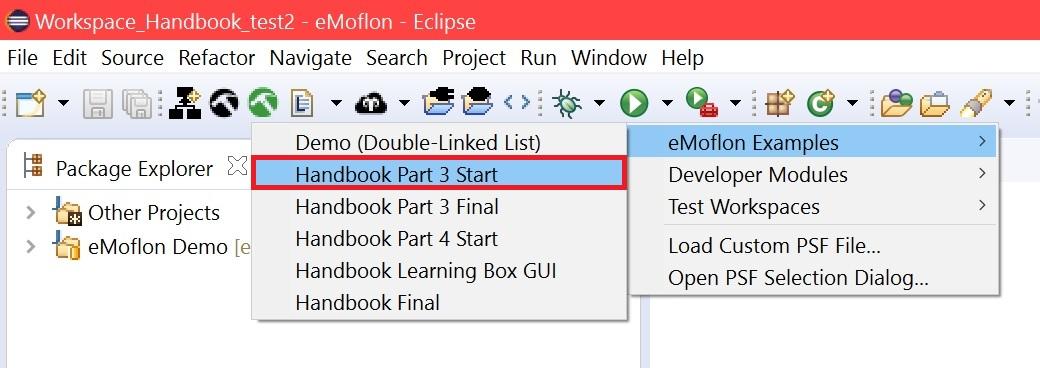
\includegraphics[width=0.75\textwidth]{eclipse_downloadWizard}
	\caption{Download a file set to get started}
	\label{fig:downloadWizard}
\end{figure}

\item[$\blacktriangleright$] Download the file package of the eMolfon specification type you'd like to learn. Remember, with the visual syntax, you'll be
using an external modeling program to craft your metamodel diagrams, then exporting the data to Eclipse for generation. With textual, you'll be working entirely
within the Eclipse IDE in the eMolfon perspective.

\newpage

\vspace*{0.5cm}

\item[$\blacktriangleright$] If your package explorer does not resemble ours in Fig.~\ref{fig:workingSets} with at least two distinct nodes, select the
small, downward facing arrow in the corner of the module window. Choose ``Working Sets'' as your ``Top Level Elements''. We use these to structure the workspace
in Eclipse.

\vspace{0.75cm}

\end{itemize}

\begin{figure}[htbp]
	\centering
  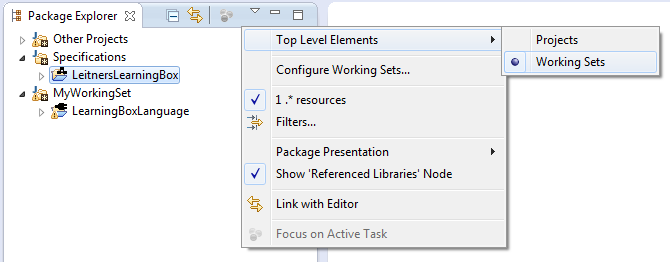
\includegraphics[width=0.9\textwidth]{eclipse_workingSets}
	\caption{Setting your Package Explorer \update}
	\label{fig:workingSets}
\end{figure}

The ``MyWorkingSet" node contains \texttt{Learn\-ing\-Box\-Lang\-uage}, which in turn contains all the code generated from your metamodel. The metamodel itself
is found in \texttt{Leit\-ners\-Learn\-ing\-Box} under ``Specifications''. The visual metamodel is a single \texttt{.eap} file, while the textual metamodel is
contained within an explicit project structure. 

These sets are not included under same node due to being different \emph{nature}s, or project types. \texttt{Learning\-Box\-Language} is your
\emph{repository project}, the Eclipse classification of a normal Java project.\footnote{For details on the project setup, review Part I, sections 4 and 5} 

\begin{itemize}

\item[$\blacktriangleright$] Inspect the files in both nodes until you feel comfortable with what you'll be working with. In particular, look at the files found
under ``gen." Each Java file has a corresponding \texttt{.impl} file, where all actionable code (such as method implementations) will be placed.\footnote{For
specific details on their contents, refer to Part II, section 5} 

\item[$\blacktriangleright$] Be sure to also review the ecore model under ``LearningBoxLanguage/model/'' and the dynamic instance found in ``instances.'' While
you can make and customize your own instance,\footnote{To learn how to make your own instance model, review Part II, section 4} we have included a small sample
in your download to help you get started.

\end{itemize}

Well, that's it! A quick review, paired with a fine download makes an excellent appetizer to SDMs. Let's get started.

% Why SDMs? Graphically, the advantage is obvious. (pictures, class diagrams, containement) textually, you can see a clear distinction between the two semantic
% types, as it separates all the actitivies into separate files, folders, and patterns.